\chapter{Evaluierung}

Um die Effektivität der erarbeiteten Lösung feststellen zu können, wird eine Evaluierung durchgeführt.
Ergänzend werden zur qualitativen Evaluierung ausgewählte Teammitglieder interviewt.

\clearpage
\section{Quantitative Evaluierung}
\subsection*{Acceptance Criteria Volatility}

\begin{savenotes}
    \begin{figure}[H]
      \centering
      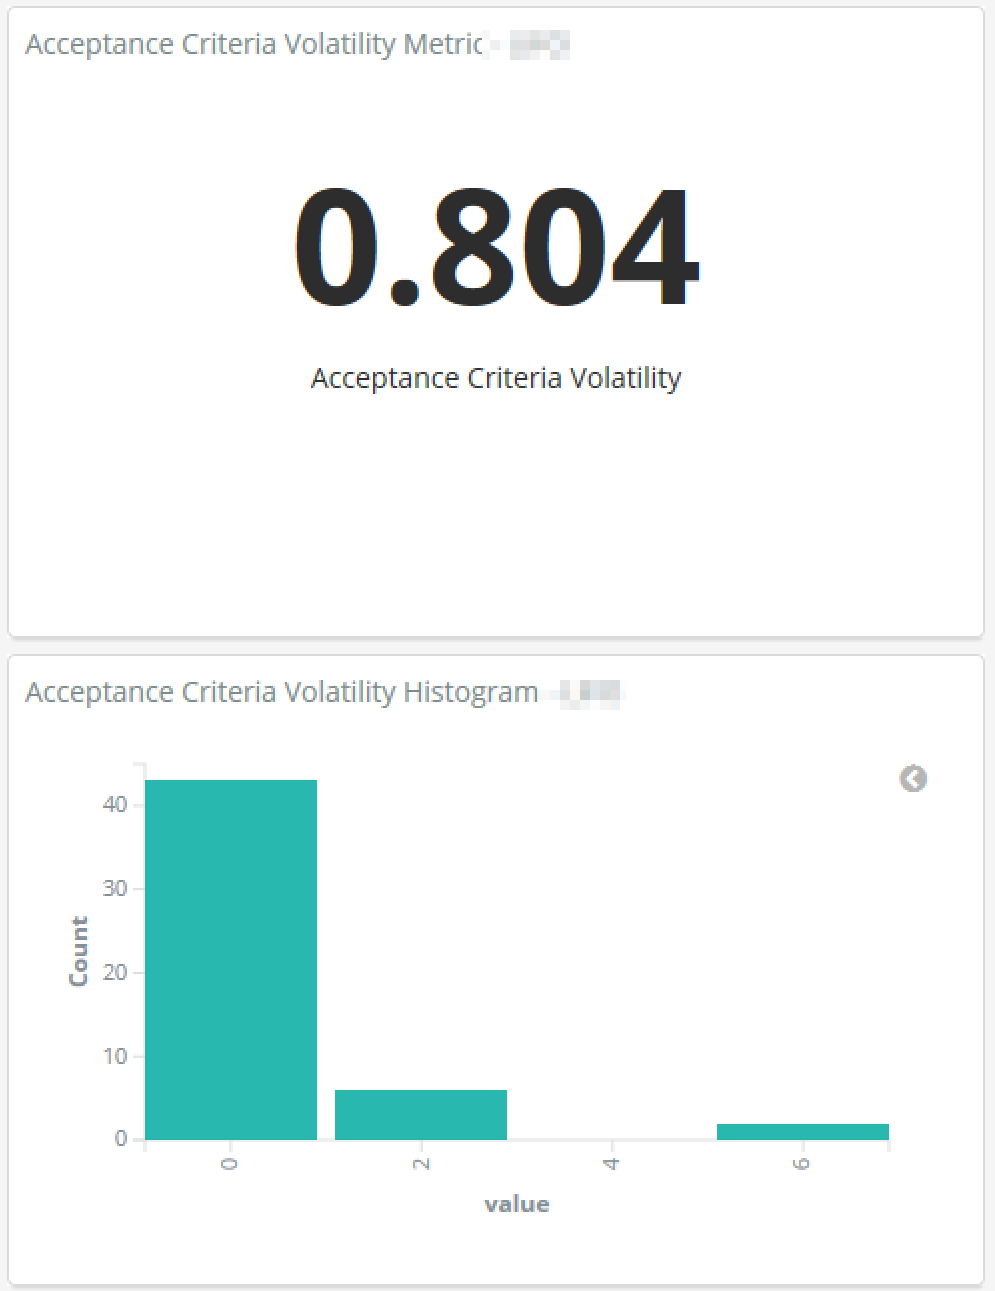
\includegraphics[width=0.7\textwidth]{img/eval-ac-volatility.png}
      \caption{Quantitative Evaluierung {-} Acceptance Criteria Volatility}\label{fig:eval_ac_volatility}
    \end{figure}
\end{savenotes}

Im Durchschnitt werden die Akzeptanzkriterien einer Aufgabe 0,8-mal geändert, was auf den ersten Blick gut aussieht.
Auch in der Verteilung im Histogramm ist zu sehen, dass ein großer Teil der Akzeptanzkriterien nach dem Erstellen der Aufgabe nicht mehr verändert wird.
Nur sehr wenige Aufgaben wurden oft verändert.
Das kann bedeuten, dass der Product-Owner inzwischen so gut versteht, was das Team von ihm verlangt, dass es zu fast keinen Änderungen mehr kommt.
Es kann aber auch bedeuten, dass die Aufgaben in den Planungsmeetings nicht kritisch hinterfragt werden.

\clearpage
\subsection*{Bug Count und Bug Rate}

\begin{savenotes}
    \begin{figure}[H]
      \centering
      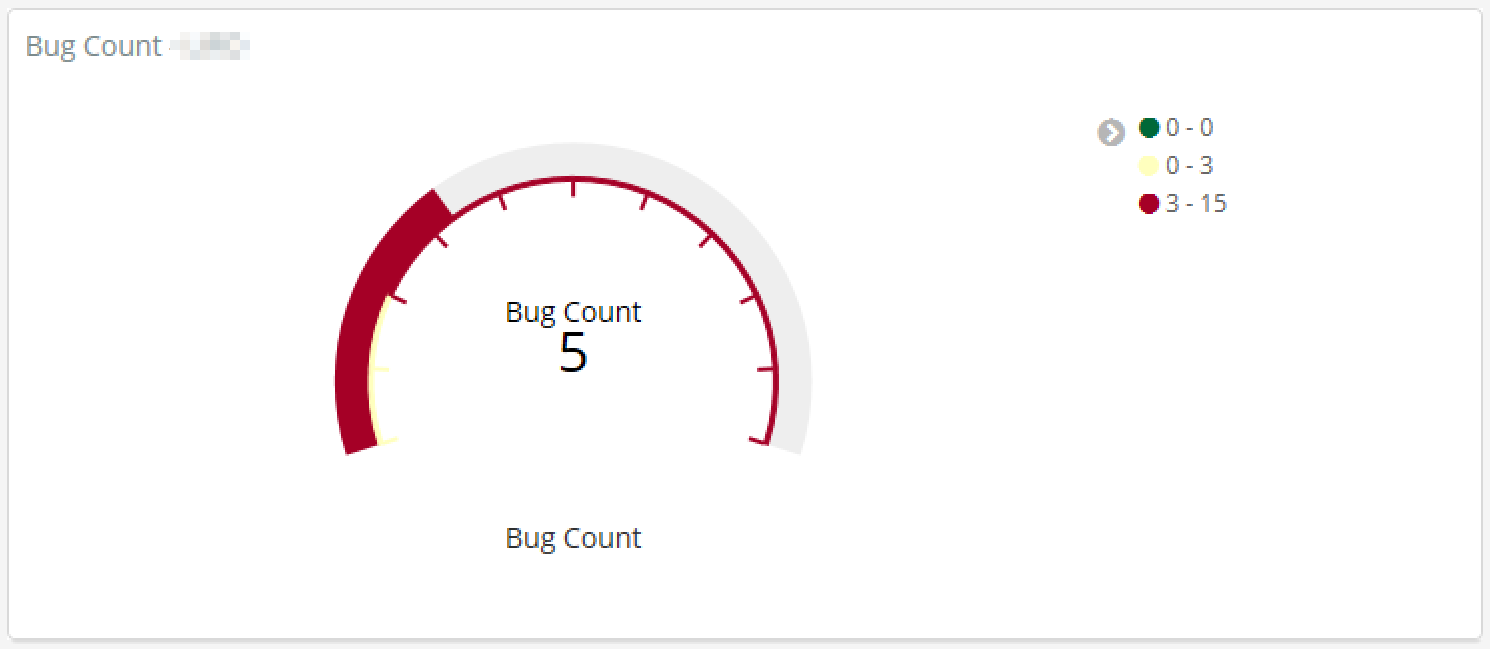
\includegraphics[width=0.9\textwidth]{img/eval-bug-count.png}
      \caption{Quantitative Evaluierung {-} Bug Count}\label{fig:eval_bug_count}
    \end{figure}
\end{savenotes}

\begin{savenotes}
    \begin{figure}[H]
      \centering
      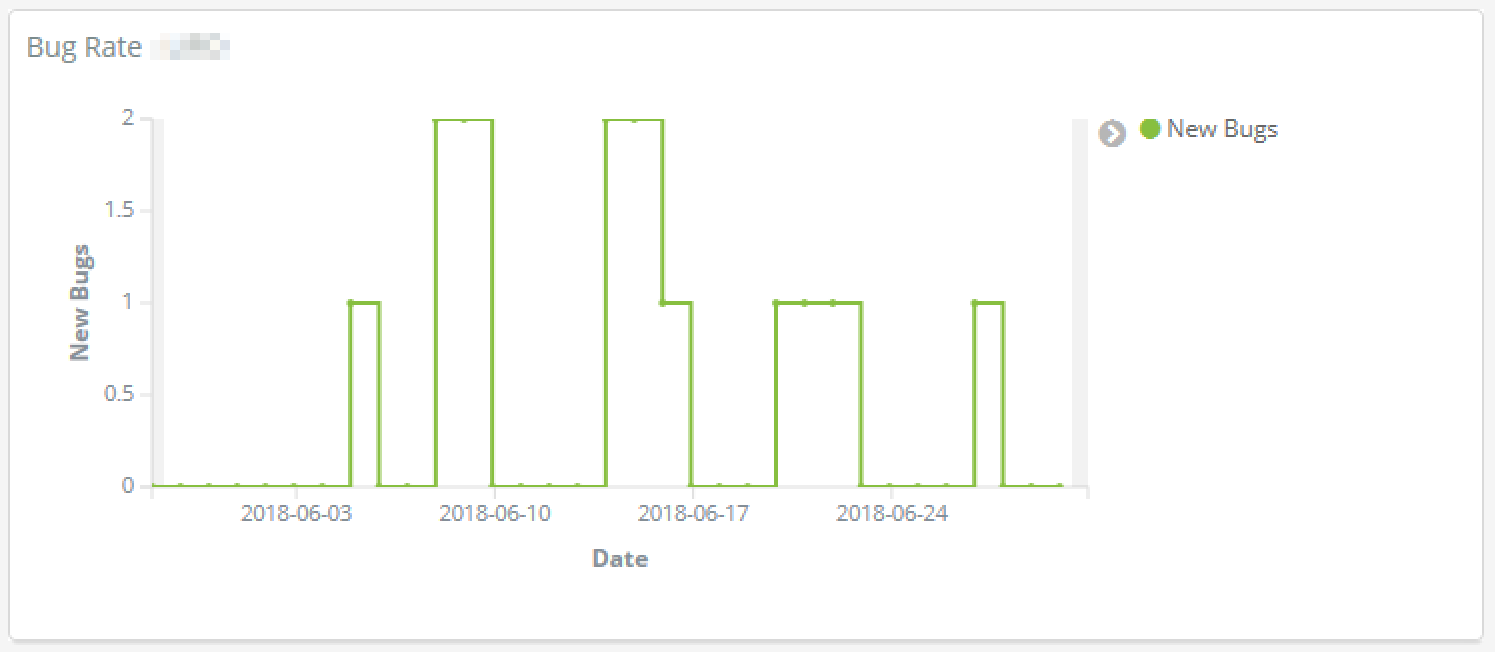
\includegraphics[width=0.9\textwidth]{img/eval-bug-rate.png}
      \caption{Quantitative Evaluierung {-} Bug Rate}\label{fig:eval_bug_rate}
    \end{figure}
\end{savenotes}

Wie in der Bug Rate in Abbildung~\ref{fig:eval_bug_rate} ersichtlich, wurden in regelmäßigen Abständen Bugs erzeugt.
Abbildung~\ref{fig:eval_bug_count} zeigt, dass noch fünf Bugs im Backlog liegen, woraus sich schließen lässt, dass Bugs im Team abgearbeitet werden.
Hier wäre noch ein Diagramm sinnvoll, wie viele Bugs pro Tag abgearbeitet werden (Bug-Fertigstellungsrate).

\clearpage
\subsection*{Burndown}

\begin{savenotes}
    \begin{figure}[H]
      \centering
      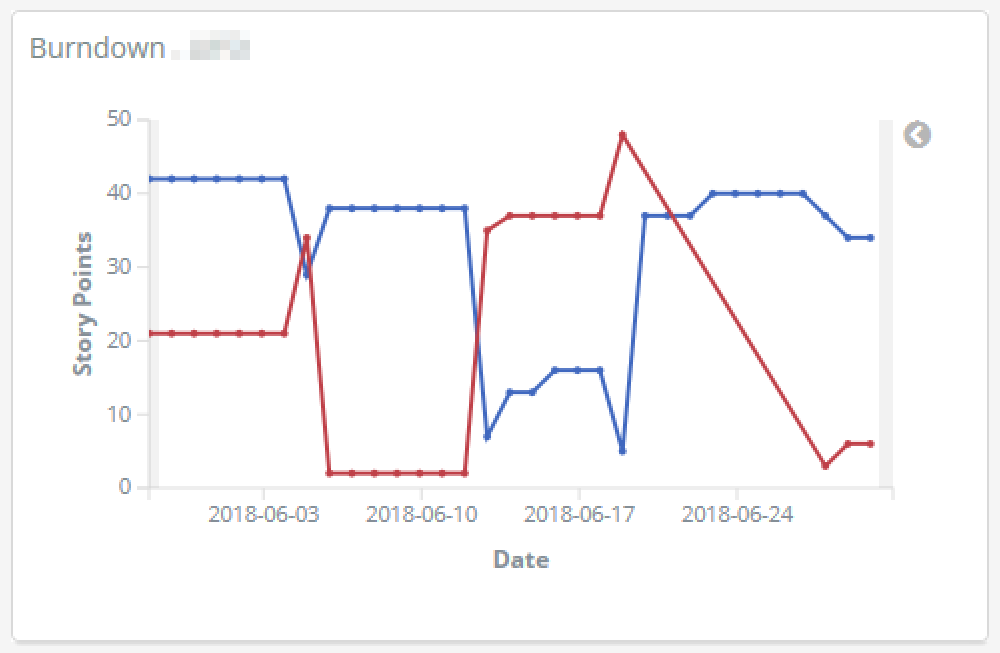
\includegraphics[width=0.8\textwidth]{img/eval-burndown.png}
      \caption{Quantitative Evaluierung {-} Burndown}\label{fig:eval_burndown}
    \end{figure}
\end{savenotes}

Die Linien zeigen die offenen (blau) und die abgeschlossenen Punkte (rot).
Das Diagramm ist sehr sprunghaft, vor allem gegen Sprintende werden plötzlich viele Punkte abgeschlossen.
Ebenfalls ersichtlich ist, dass während dem Sprint immer wieder Punkte dazukommen.
Hier besteht noch viel Verbesserungspotential. Bei den abgeschlossenen Punkten (rot) ist ebenfalls ersichtlich, dass ein paar Datenpunkte fehlen.
Das kann ein Problem der Agile-Metrics-Software sein und muss genauer analysiert werden.

\clearpage
\subsection*{Coverage}

\begin{savenotes}
    \begin{figure}[H]
      \centering
      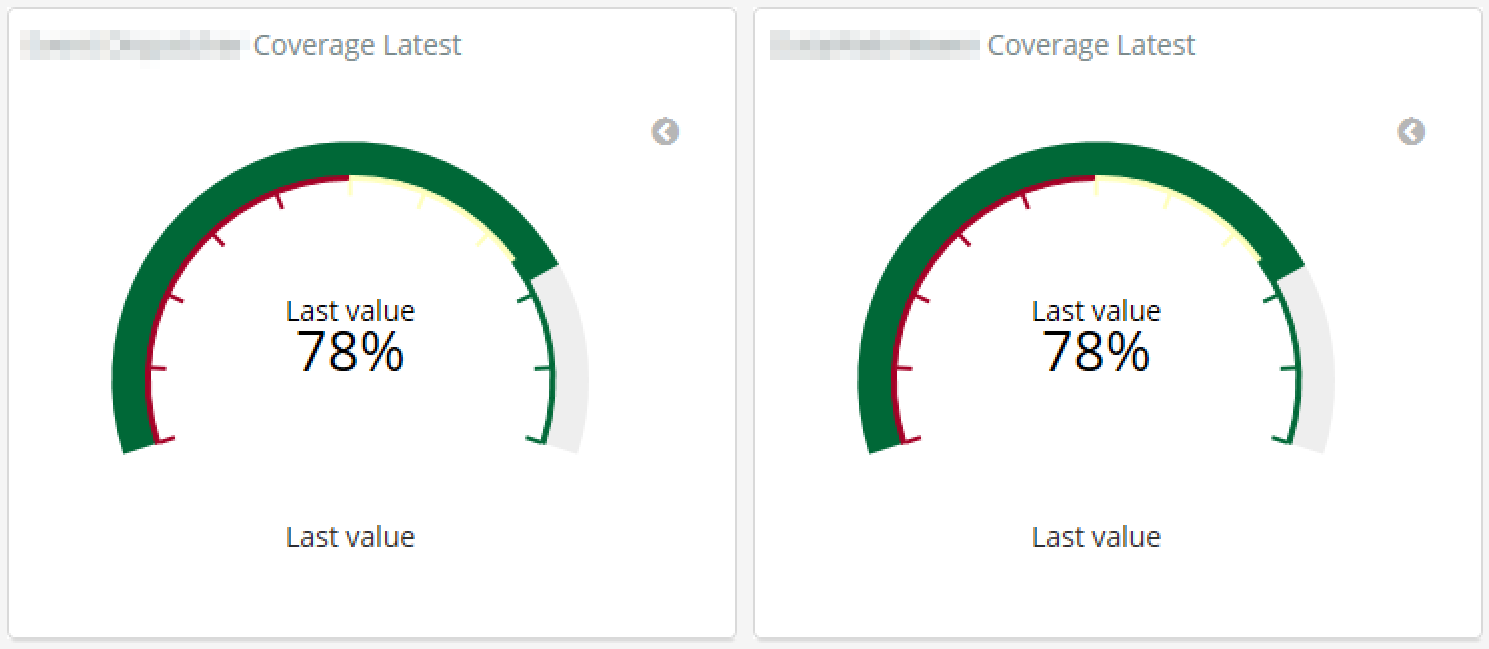
\includegraphics[width=0.8\textwidth]{img/eval-coverage-1.png}
      \caption{Quantitative Evaluierung {-} Coverage der kritischen Komponenten}\label{fig:eval_coverage_1}
    \end{figure}
\end{savenotes}

\begin{savenotes}
    \begin{figure}[H]
      \centering
      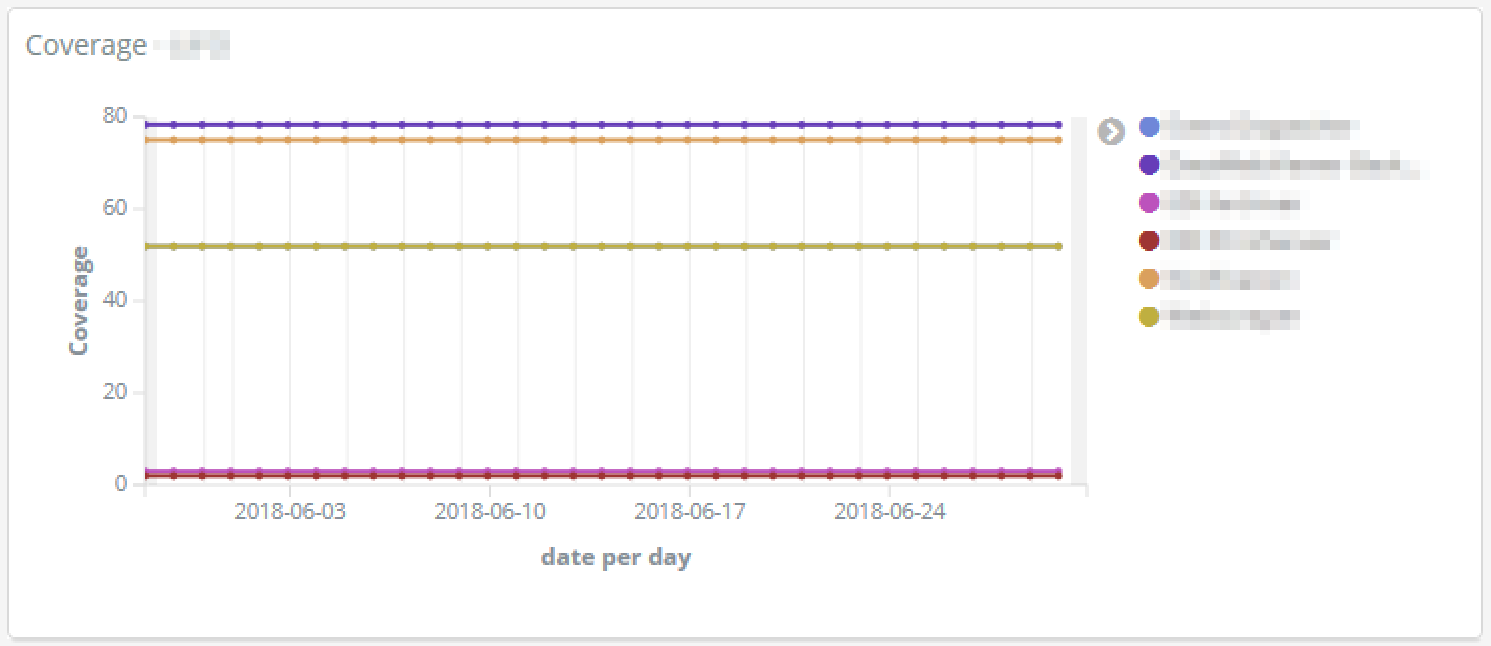
\includegraphics[width=0.8\textwidth]{img/eval-coverage-2.png}
      \caption{Quantitative Evaluierung {-} Coverage aller Komponenten}\label{fig:eval_coverage_2}
    \end{figure}
\end{savenotes}

Bei der Coverage hat sich im Testzeitraum nichts verändert.
Zwei der Hauptkomponenten sind mit 78\% Testabdeckung auf einem guten Niveau, wie in Abbildung~\ref{fig:eval_coverage_1} ersichtlich.
Andere Komponenten befinden sich fast bei null Prozent, wie in Abbildung~\ref{fig:eval_coverage_2} ersichtlich, und haben daher noch viel Verbesserungspotential.

\clearpage
\subsection*{Cumulative Flow}

\begin{savenotes}
    \begin{figure}[H]
      \centering
      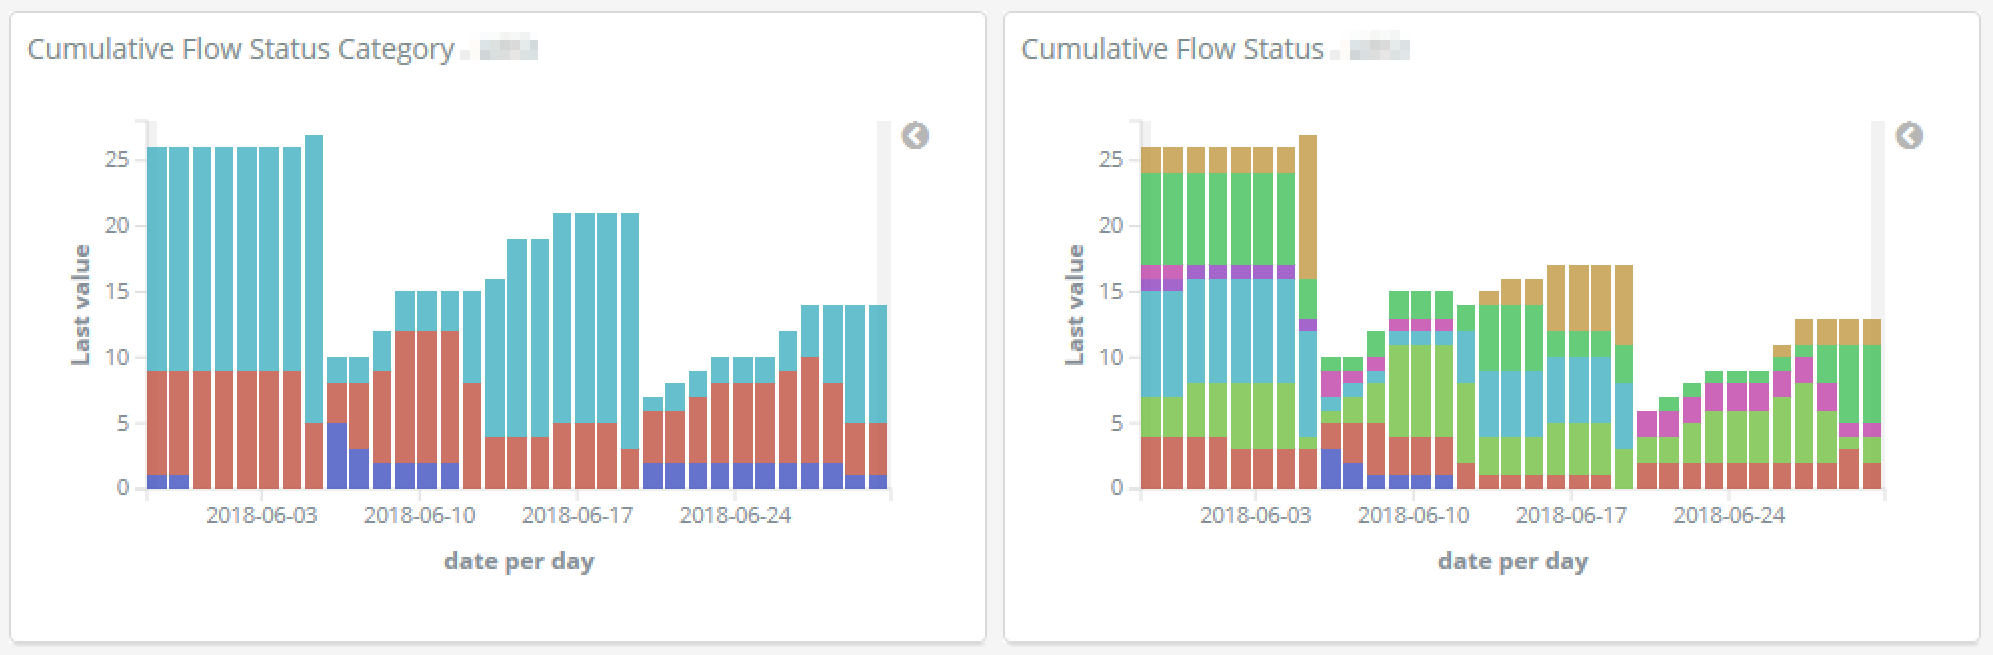
\includegraphics[width=1.0\textwidth]{img/eval-cumulative.png}
      \caption{Quantitative Evaluierung {-} Cumulative Flow}\label{fig:eval_cumulative}
    \end{figure}
\end{savenotes}

Anhand des Cumulative Flow, vor allem dem der Status-Kategorien, ist der Fortschritt des Sprint-Backlogs besser zu erkennen.
Anders als im Burndown-Diagramm ist hier ein kontinuierlicher Fortschritt ersichtlich.
Auffallend ist, dass bei jedem Sprint im Testzeitraum nicht abgeschlossene Punkte in den nächsten Sprint übernommen wurden.

\clearpage
\subsection*{Labels}

\begin{savenotes}
    \begin{figure}[H]
      \centering
      
\includegraphics[width=0.8\textwidth]{img/eval-labels.png}
      \caption{Quantitative Evaluierung {-} Labels}\label{fig:eval_labels}
    \end{figure}
\end{savenotes}

Die Labels wurden vom Team bei der Retrospektive für jede abgeschlossene Aufgabe vergeben.
Für die Arbeit vergaben sie die Labels `WorkPlus' (Arbeit gut verlaufen) und `WorkMinus' (Arbeit schlecht verlaufen) und für die Aufbereitung wurde `IssuePlus' (Aufgabe gut aufbereitet) und `IssueMinus' (Aufgabe schlecht aufbereitet) vergeben.
Dadurch kann das subjektive Empfinden des Teams während eines Sprints oder eines bestimmten Zeitraums dargestellt werden.
In diesem Fall wurde im Testzeitraum die Arbeit als durchwegs gut und die Aufbereitung als mehrheitlich gut empfunden.

\clearpage
\subsection*{Lead Time}

\begin{savenotes}
    \begin{figure}[H]
      \centering
      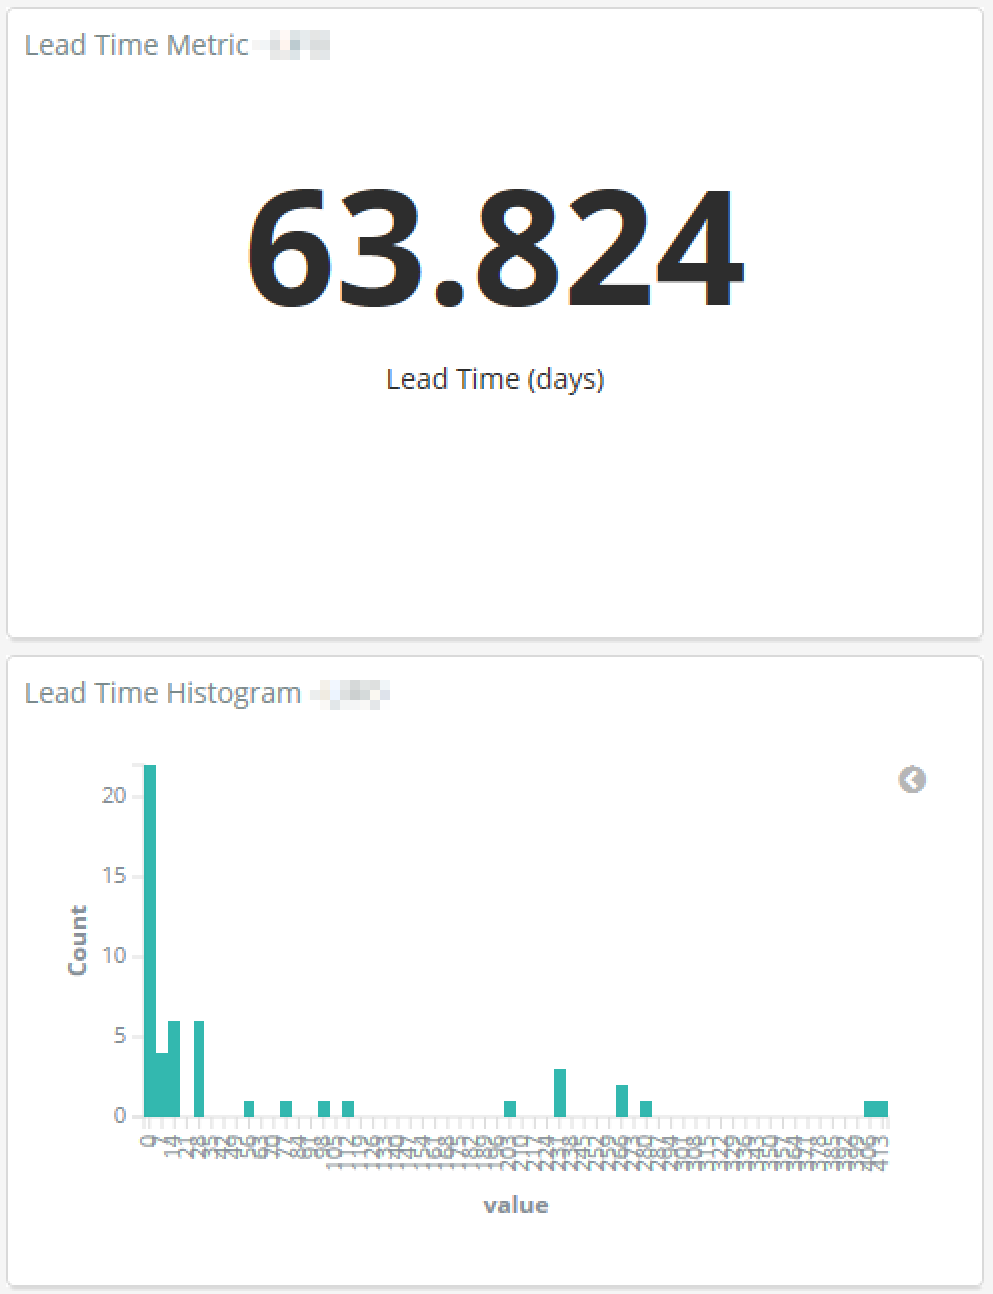
\includegraphics[width=0.8\textwidth]{img/eval-lead.png}
      \caption{Quantitative Evaluierung {-} Lead Time}\label{fig:eval_lead_time}
    \end{figure}
\end{savenotes}

Bei der Lead Time ist das Histogramm sehr hilfreich, da hier die Ausreißer sehr gut ersichtlich sind.
Nicht nur, dass der größte Teil der Aufgaben am selben Tag abgeschlossen wurde, an dem sie erstellt wurden, sondern auch, dass gewisse Aufgaben mehr als 100 Tage lang, manche sogar bis zu 400 Tage bis zur Fertigstellung benötigten.
Leider fehlt hier noch eine Möglichkeit, solche Ausreißer noch genauer zu analysieren.

\clearpage
\subsection*{Recidivism}

\begin{savenotes}
    \begin{figure}[H]
      \centering
      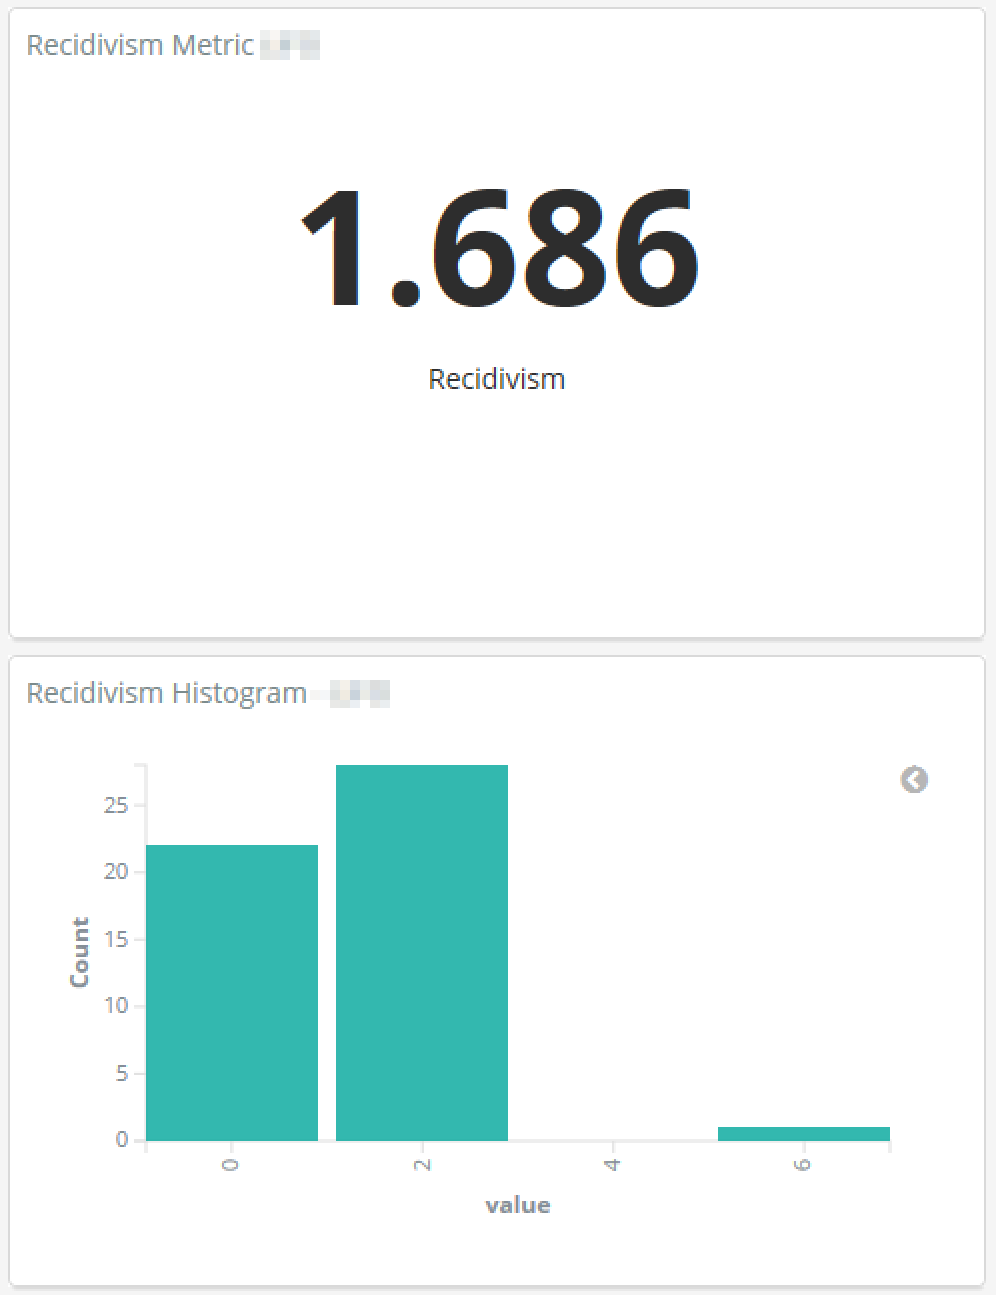
\includegraphics[width=0.8\textwidth]{img/eval-recidivism.png}
      \caption{Quantitative Evaluierung {-} Recidivism}\label{fig:eval_recidivism}
    \end{figure}
\end{savenotes}

Auch bei der Rückfälligkeit gibt es noch Verbesserungspotential.
Die Metrik zeigt, dass im Testzeitraum eine Aufgabe im Schnitt 1,6-mal im Arbeitsfluss rückwärts ging.
Im Histogramm ist auch in der Verteilung zu erkennen, dass die meisten Aufgaben zweimal im Arbeitsfluss rückwärts gingen.
Eine Aufgabe ging sogar 6-mal rückwärts und auch hier fehlt noch eine Detailansicht, um solche Ausreißer zu identifizieren.

\clearpage
\subsection*{Test Execution Time}

\begin{savenotes}
    \begin{figure}[H]
      \centering
      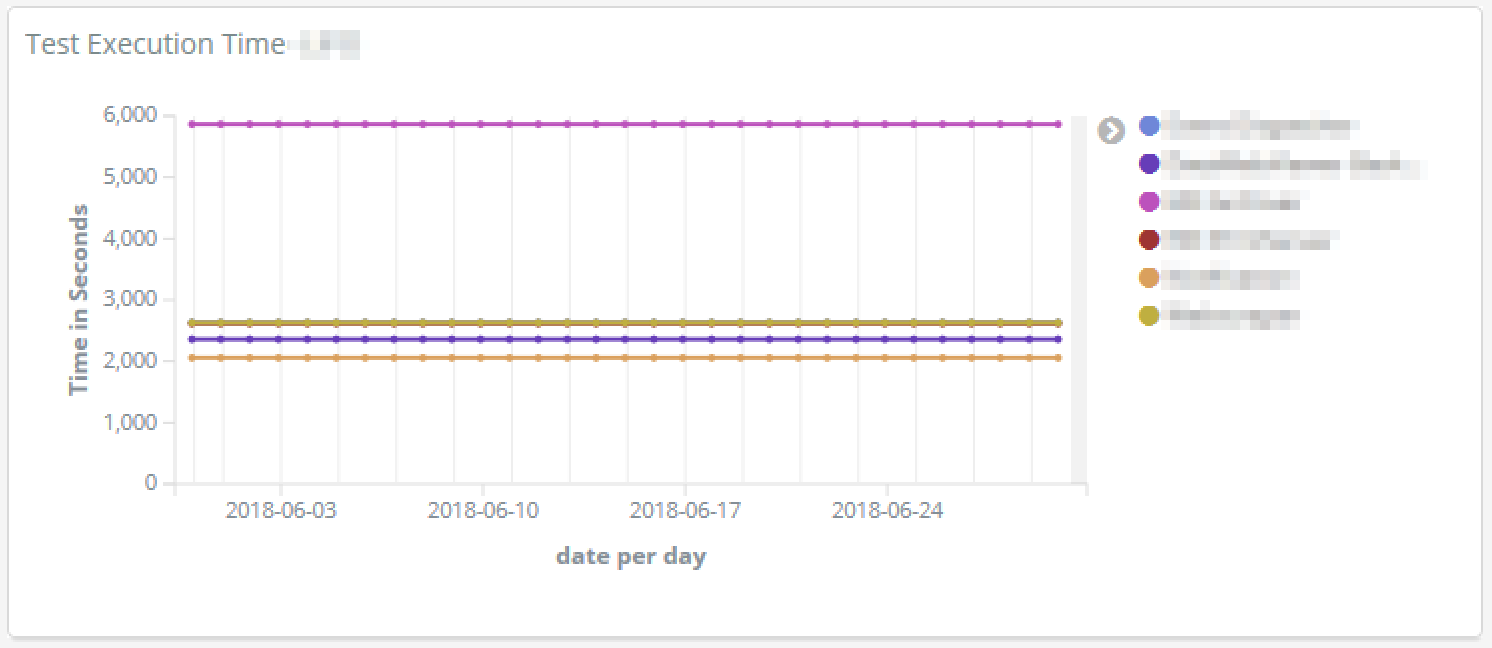
\includegraphics[width=1.0\textwidth]{img/eval-test-exec.png}
      \caption{Quantitative Evaluierung {-} Test Execution Time}\label{fig:eval_test_execution}
    \end{figure}
\end{savenotes}

Die Laufzeit der Tests ist noch ausbaufähig.
Sie blieb zwar im gesamten Testzeitraum konstant, was aber auch bedeuten kann, dass in diesem Zeitraum keine neuen Tests geschrieben wurden.
Hier kann oft schon viel durch parallele Testausführung erreicht werden.

\clearpage
\subsection*{Velocity}

\begin{savenotes}
    \begin{figure}[H]
      \centering
      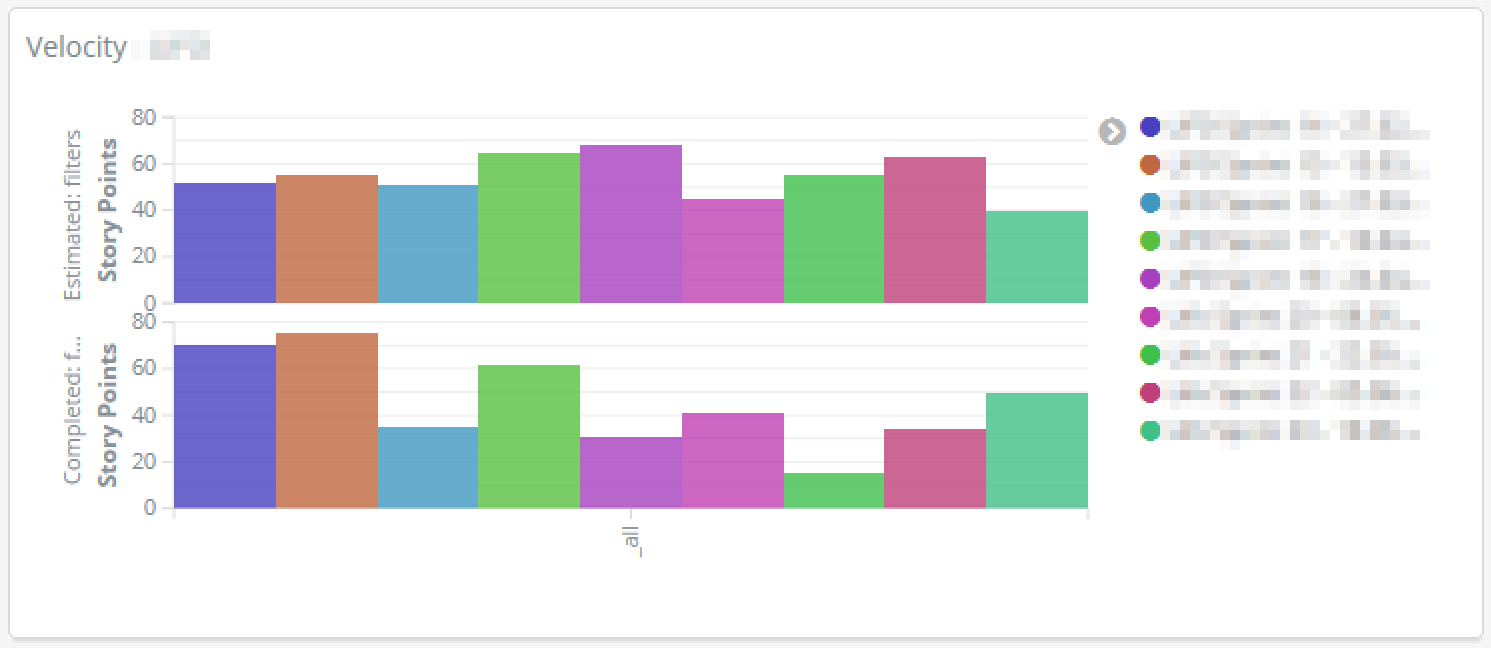
\includegraphics[width=1.0\textwidth]{img/eval-velocity.png}
      \caption{Quantitative Evaluierung {-} Velocity}\label{fig:eval_velocity}
    \end{figure}
\end{savenotes}

\begin{savenotes}
    \begin{figure}[H]
      \centering
      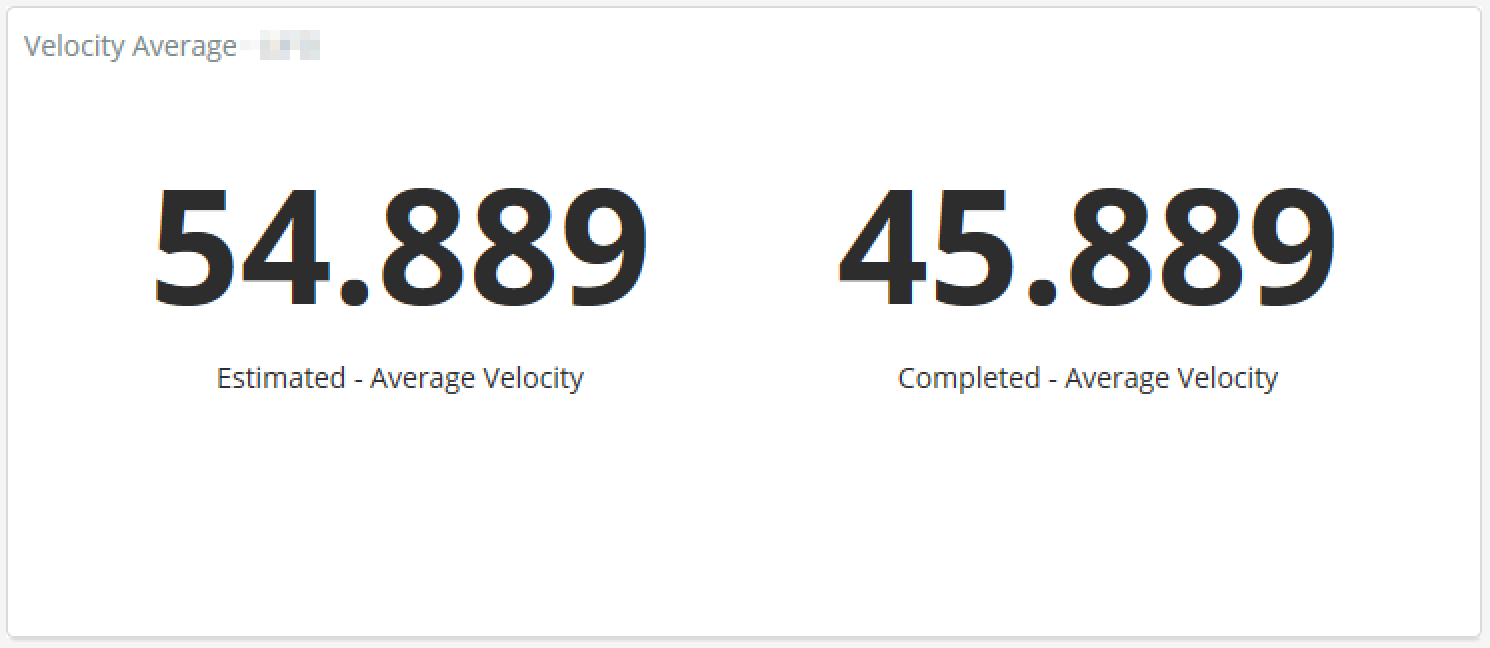
\includegraphics[width=1.0\textwidth]{img/eval-velocity-avg.png}
      \caption{Quantitative Evaluierung {-} Velocity Durchschnitt}\label{fig:eval_velocity_avg}
    \end{figure}
\end{savenotes}

Velocity ist die einzige Metrik, die für mehrere Sprints rückwirkend generiert wurde.
Abbildung~\ref{fig:eval_velocity} zeigt, dass im letzten Sprint, in dem das Dashboard aktiv war, wieder mehr Punkte abgearbeitet wurden als anfangs geschätzt.
In den zwei Sprints zuvor wurde mehr geschätzt als abgeschlossen.
Beim Durchschnitt in Abbildung~\ref{fig:eval_velocity_avg} ist es das Ziel, die beiden Kennzahlen über die Zeit möglichst gut anzunähern.

\clearpage
\subsection*{Issue Volume}

\begin{savenotes}
    \begin{figure}[H]
      \centering
      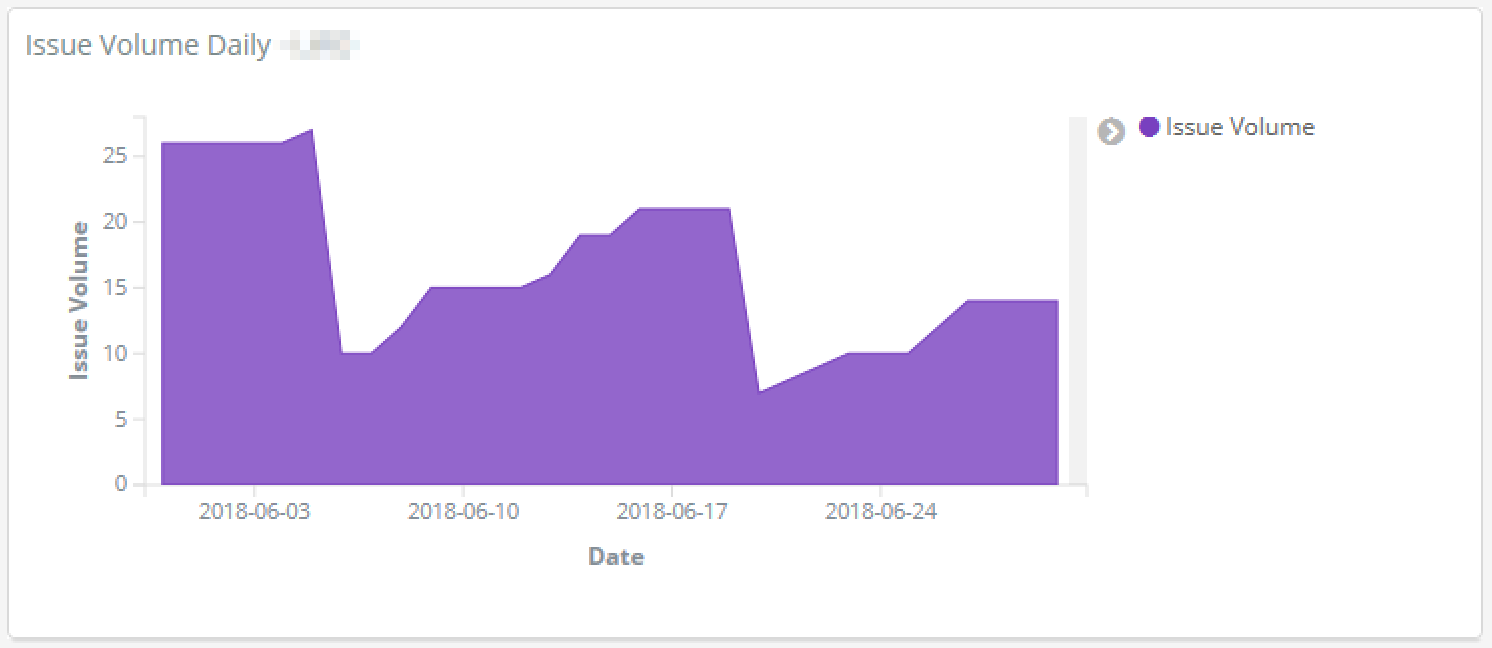
\includegraphics[width=1.0\textwidth]{img/eval-volume.png}
      \caption{Quantitative Evaluierung {-} Issue Volume}\label{fig:eval_issue_volume}
    \end{figure}
\end{savenotes}

\begin{savenotes}
    \begin{figure}[H]
      \centering
      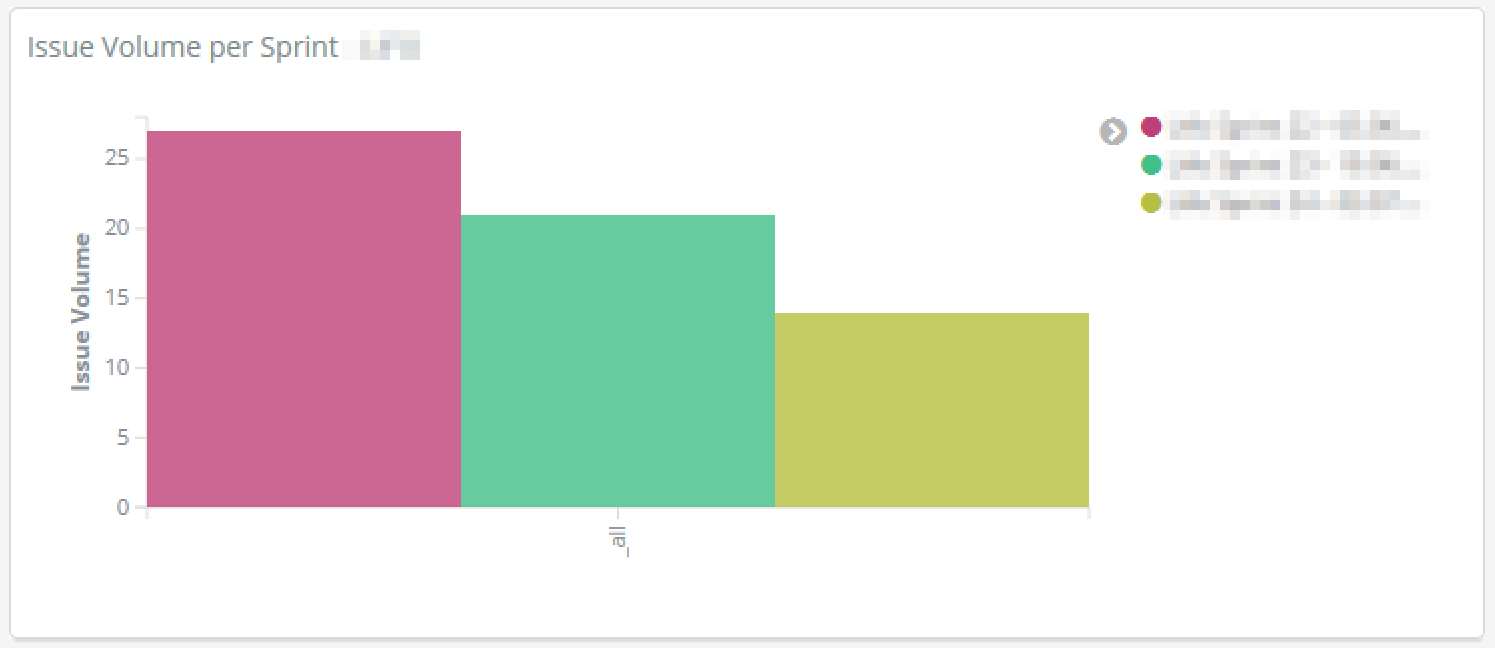
\includegraphics[width=1.0\textwidth]{img/eval-volume-total.png}
      \caption{Quantitative Evaluierung {-} Issue Volume Total}\label{fig:eval_issue_volume_total}
    \end{figure}
\end{savenotes}

Das absolute Issue Volume hat sich in den drei Sprints des Testzeitraums kontinuierlich verkleinert, wie in Abbildung~\ref{fig:eval_issue_volume_total} ersichtlich.
Trotzdem zeigt Abbildung~\ref{fig:eval_issue_volume}, dass während jedem Sprint immer wieder neue Aufgaben zum Sprint-Backlog hinzugefügt wurden.

\clearpage
\subsection*{Zusammenfassung}

In der quantitativen Evaluierung sind bei einigen Metriken schon Tendenzen erkennbar.
Ob die Verbesserungen allerdings durch das Dashboard eingetreten sind, ist in diesem kurzen Zeitraum von nicht ganz drei Sprints nicht eindeutig zu sagen.
Um eine solche Aussage treffen zu können, müsste das Team länger begleitet werden, um auch Korrelationen zwischen den Metriken aufzeigen zu können.
Was aber eindeutig gesagt werden kann, ist, dass viele der Metriken Schwachstellen aufzeigen konnten und somit gezeigt werden konnte, dass die Auswahl an Metriken richtig getroffen wurde.
Einige Schwachstellen, wie das Anzeigen von mehr Details zu den Metriken, könnten noch behoben werden, um das Dashboard effizienter zu machen.

\clearpage
\section{Qualitative Evaluierung}

Zur qualitativen Evaluierung werden Interviews mit dem Scrum-Master, dem Product-Owner und einer Entwicklerin geführt.
Das ermöglicht einen Einblick aus Managementsicht (Product-Owner) und aus Prozesssicht (Scrum-Master und Entwicklerin), welche womöglich ganz unterschiedliche Anforderungen an die Lösung stellen.
Dabei soll herausgefunden werden, ob die richtigen Metriken ermittelt wurden und welche Metriken als besonders nützlich angesehen werden.
Ebenfalls wird nach einer nachweisbaren und spürbaren Qualitätsverbesserung gefragt.
Interessant ist auch noch, wann und wie das Dashboard genutzt wird und wie es um die Benutzbarkeit steht.

\subsection{Interview-Fragen}

Folgende Interviewfragen sollen helfen, den roten Faden im Gespräch zu behalten.
Als Einstieg wird das Dashboard geöffnet, um es während dem Gespräch immer sichtbar vor sich zu haben.

\begin{enumerate}
    \item Wird das Dash\-board von dir genutzt? Wenn ja, wann und wie nutzt du das Dashboard?
    \item Wie ist der Zugang und die Bedienbarkeit des Dashboards?
    \item Ist das Dashboard übersichtlich und klar eingeteilt?
    \item Rückblickend gesehen, wurden die richtigen Metriken ermittelt und auf dem Dashboard visualisiert?
    \item Welche Metriken auf dem Dashboard sind besonders nützlich oder werden oft genutzt?
    \item Ist bereits eine Qualitätsverbesserung im Prozess oder in einem Produkt spürbar? Oder sogar nachweisbar?
    \item Gibt es aus deiner Sicht Verbesserungspotential? Wo liegen aus deiner Sicht die Schwächen dieser Lösung?
\end{enumerate}

Die Interviews wurden mit Zustimmung der Interviewten aufgezeichnet, ein Transkript befindet sich in Anhang~\ref{appendix:transcript}.

\clearpage
\subsection{Interview-Antworten}

Auffallend bei den Antworten sind die unterschiedlichen Sichten auf das Dashboard.
Während der Product-Owner das Dashboard mehr für Werbezwecke genutzt hat, um andere Abteilungen auf die Möglichkeit von Metriken aufmerksam zu machen, hat es der Scrum-Master eher für die Langzeit-Sicht des Teams genutzt und seinen Fokus auf die Verbesserung des Prozesses gelegt.
Die Entwicklerin wiederum hatte den Fokus auf die kurzfristigen Metriken, wie den Bug Count, um schnell auf Probleme reagieren zu können.
Genutzt wurde es daher von allen Befragten, wichtiger ist aber, dass alle einen Nutzen darin sahen und es für sich bestmöglich nutzen können.
Bei der Bedienbarkeit sind einzelne Schwächen aufgetaucht, vor allem was die Detailansicht von Kennzahlen betrifft.
Die Einteilung der Metriken auf dem Dashboard wurde von allen als übersichtlich empfunden, eine Kennzeichnung der betroffenen Rollen (Scrum-Master, Product-Owner oder Entwicklerinnen) wäre eventuell noch sinnvoll.
Auch eine genauere Beschreibung der Ziele und gewisser Metriken könnte Missverständnisse verhindern.
Die Auswahl der Metriken wurde als gut empfunden, manche Metriken machen erst Sinn, wenn sie mit anderen kombiniert werden.
Diese Kombination von Metriken war vor allem dem Scrum Master bewusst und wird in absehbarer Zukunft auch noch so umgesetzt.
Welche Metriken als besonders nützlich angesehen werden, hängt stark von der Rolle ab.
Wie bereits anfangs erwähnt, interessiert sich die Entwicklerin mehr für die kurzzeitigen Metriken, die unmittelbar Feedback zur Entwicklung liefern, während das Interesse des Scrum-Masters und Product-Owners mehr bei den Langzeit-Metriken liegt.
Eine Qualitätsverbesserung ist noch nicht eindeutig ersichtlich, da es ein noch zu kurzer Zeitraum ist, um darüber Aussagen treffen zu können.
Was aber von der Entwicklerin als spürbar erwähnt wurde, ist der Umgang mit den Bugs, die nun frühzeitig erkannt und abgearbeitet werden können.
Verbesserungspotential sehen alle noch bei der Nutzung der Metriken, was aber auch vor allem auf den zu kurzen Zeitraum der Tests rückführbar ist.
Einige gute Vorschläge, wie das Beschreiben von Zielen, eine bessere Kategorisierung nach Rollen und das Interesse an neuen Metriken zeigen aber, dass das Dashboard durchaus genutzt und das Ziel dahinter, das Ganze als Werkzeug für das gesamte Team zu nutzen, bereits erkannt wurde.
